\documentclass[11pt]{article}
\setcounter{tocdepth}{3}
\setcounter{secnumdepth}{3}

\usepackage[english,italian]{babel}
\usepackage[a4paper, top=2cm, bottom=1.5cm, left=2cm, right=2cm]{geometry}
\usepackage{float}
\usepackage{ltablex}
\usepackage{titling}
\usepackage{blindtext}
\usepackage[utf8]{inputenc}
\usepackage[T1]{fontenc}
\usepackage{xcolor}

\usepackage{natbib}
\usepackage{graphicx}

\usepackage{geometry}
\usepackage[italian]{babel}
\usepackage{tabularx}
\usepackage{longtable}
\usepackage{hyperref}
\usepackage[bottom]{footmisc}
\usepackage{fancyhdr}
\usepackage{titlesec}
\usepackage{amsmath, amssymb}
\usepackage{array}
\usepackage{graphicx}
\usepackage{url}
\usepackage{comment}
\usepackage{eurosym}


\begin{document}

\thispagestyle{empty}
	\begin{titlepage}
		\begin{center}
			
\includegraphics[scale = 0.05]{Res/logo_unipd.png}\\
			\bigskip
			\large \textbf{Università degli Studi di Padova} \\
			\vfill
			
\includegraphics[scale = 0.7]{Res/BugPharma_Logo.png}\\
			\huge \textbf{Gruppo Bug Pharma} \\
			\vfill
			\large \texttt{bugpharma10@gmail.com}
			\vfill
			\Huge \textbf{Valutazione Capitolati 2021/2022}\\
			
			\vfill
			
			\large
			\begin{tabular}{r|l}
				\textbf{Approvazione} &  -\\
				\textbf{Redazione} &  \parbox[t]{3.5cm}{Lorenzo Piran \\ Michele Masetto \\ Sara Nanni \\ Andrea Salmaso}\\
				\textbf{Verifica} &  -\\
				\textbf{Stato} & Redatto \\
				\textbf{Uso} & Esterno
			\end{tabular}
			\vfill
			
		\end{center}
	\end{titlepage}

\tableofcontents

\newpage


\section{Valutazione del capitolato scelto}
\subsection{Capitolato C5 - Login Warrior}

    \subsubsection{Informazioni generali}
    \begin{itemize}
        \item \textbf{Nome}: Login Warrior;
        \item \textbf{Proponente}: Zucchetti S.p.A.;
        \item \textbf{Committente}: Prof. Tullio Vardanega e Prof. Riccardo Cardin.
    \end{itemize}
    
    \subsubsection{Descrizione}
    Il capitolato ha per oggetto l'affidamento della fornitura per la realizzazione di un'applicazione di visualizzazione di dati di
    login a supporto della fase esplorativa (\textit{EDA}) del riconoscimento e distinzione di attività lecite o illecite che possono
    essere svolte all'interno delle procedure cloud fornite dall'azienda ai propri clienti.
    
    Tale applicazione fornirà quindi ausilio ai data analyst, i quali, partendo da un insieme di dati contenuti in un file
    \texttt{CSV}, potranno risalire a grafici e dataset che forniranno un immediato riscontro visivo sulla presenza o meno di attività
    illecite.
    
    \subsubsection{Dominio}
        \paragraph{Dominio Applicativo}~\\
        
        \noindent
        Il capitolato si colloca nell'ambito della creazione di un applicativo web che permetta l'importazione di dataset presenti in
        file \texttt{CSV} e la visualizzazione di varie tipologie di grafico basate su di essi.
        Gli utenti finali sono quindi data analyst che analizzeranno gli accessi alle procedure cloud messe a disposizione dall'azienda.
        
        \paragraph{Dominio Tecnologico}~\\
        
        \noindent
        Per lo svolgimento del capitolato e per la creazione dell'applicativo web vengono richieste conoscenze in ambito web, in
        particolare:
        \begin{itemize}
            \item \textit{HTML}: per la struttura ed il markup della pagina;
            \item \textit{CSS}: per la presentazione visiva dell'applicativo web;
            \item \textit{JavaScript}: per il comportamento e il trattamento dei dati;
            \item \textit{D3.js}: libreria \textit{JavaScript} per la manipolazione di documenti basati sui dati;
        \end{itemize}
    
    \subsubsection{Motivazione della scelta}
        \paragraph{Aspetti positivi}
        \begin{itemize}
            \item Le tecnologie e la libreria proposta da Zucchetti S.p.A sono strumenti molto diffusi e utilizzati nell'ambito della
            gestione e presentazione dei dati, con conseguente esaustività della documentazione;
            \item Consistente set di dati su cui effettuare test;
            \item Disponibilità mostrata dall'azienda all'aiuto e alla collaborazione con il gruppo, evidenziando quanto un eventuale
            risultato positivo possa essere effettivamente utilizzato in futuro;
            \item Possibilità di ottenere nuove conoscenze spendibili in futuro nel mondo lavorativo;
            \item Possibilità di applicare gli insegnamenti avuti dal corso parallelo di Tecnologie Web.
        \end{itemize}
        \paragraph{Fattori critici}
        \begin{itemize}
            \item La maggior parte degli elementi del gruppo ha poca o nulla familiarità con le tecnologie proposte;
            \item Il dover creare grafici puliti e chiari per permettere la veloce individuazione di un accesso sospetto
            \item confrontarsi con librerie e algoritmi di ML.
        \end{itemize}
    
    \subsubsection{Conclusioni}
    Il buon esito degli incontri avuti con il referente di Zucchetti S.p.A., Gregorio Piccoli, e le accortezze prese dall'azienda,
    nonché la possibilità di utilizzare tecnologie interessanti e di affrontare un argomento molto stimolante per tutti gli elementi del
    gruppo, ha portato alla scelta del capitolato in oggetto.
    
    \begin{figure}[h!]
        \centering
        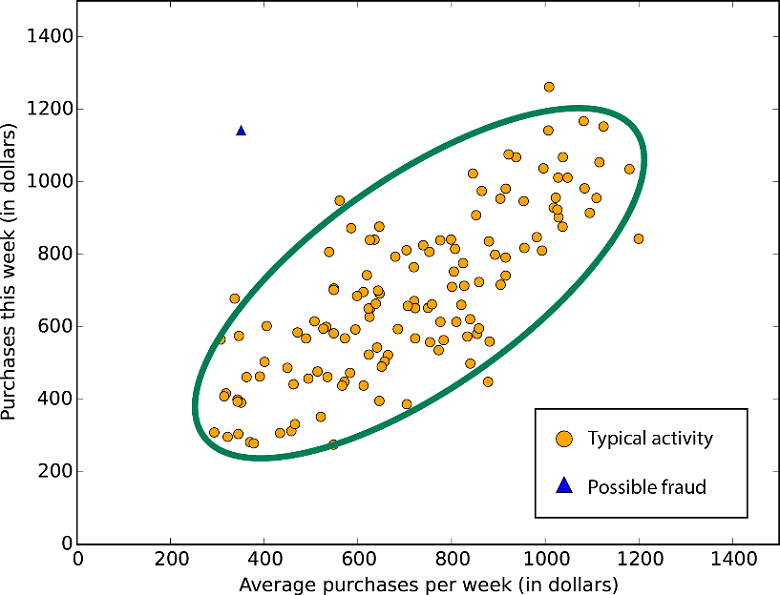
\includegraphics[scale=0.4]{Res/LoginWarrior.png}
        \caption{Grafico accesso utenti}
        \label{zucchetti}
    \end{figure}

\newpage


\section{Valutazioni sui capitolati rimanenti}
\subsection{Capitolato C1: Bot4Me}

    \subsubsection{Informazioni generali}
    \begin{itemize}
        \item \textbf{Nome}: Bot4Me;
        \item \textbf{Proponente}: Imola Informatica S.p.A.;
        \item \textbf{Committente}: Prof. Tullio Vardanega e Prof. Riccardo Cardin.
    \end{itemize}
    
    \subsubsection{Descrizione}
    Il capitolato si focalizza sulla realizzazione di un'applicazione chatbot in grado di interpretare un flusso testuale,
    con lo scopo di aiutare i dipendenti a familiarizzare con gli strumenti e con il contesto aziendale.
    
    \begin{figure}[h!]
        \centering
        
\includegraphics[scale=0.3]{Res/BotMe.png}
        \caption{Logo Bot4Me}
        \label{Bot4Me}
    \end{figure} 
    
    \subsubsection{Dominio}
        \paragraph{Dominio Applicativo}~\\

        Il capitolato vuole soddisfare l'esigenza del poter consuntivare le attività giornaliere dei dipendenti aziendali in un
        periodo storico ove il Covid-19 ha costretto a mutare radicalmente modi di fare e abitudini delle persone.
        L'applicazione permetterebbe quindi di:
		\begin{itemize}
			\item Effettuare operazioni di check-in e check-out;
			\item Inserire di un consuntivo dell'attività giornaliera;
			\item Creare nuove riunioni;
			\item Aprire ticket di tracciamento di bug o progetti;
			\item Ricercare dei documenti sul repository aziendale;
			\item Aprire il cancello della sede aziendale.			
		\end{itemize}		        
		
        \paragraph{Dominio Tecnologico}~\\
        
        Per lo svolgimento del capitolato e per la creazione dell'applicativo sono richieste la conoscenza e la padronanza
        delle seguenti tecnologie:
        \begin{itemize}
            \item \textit{API di EMT}: per la registrazione dell'ingresso e l'inserimento di attività;
            \item \textit{Protocollo MQTT}: per la gestione dell'apertura del cancello (requisito opzionale);
            \item \textit{API Redmine}: per effettuare le operazioni di inserimento di un nuovo ticket;
        \end{itemize}
    
    \subsubsection{Fattori Critici}
    Qui di seguito i fattori critici sui quali si è soffermato il gruppo e che hanno fatto desistere dalla scelta del capitolato in
    oggetto:
    	\begin{itemize}
            \item Presenza di molti requisiti obbligatori, i quali richiedono una certa praticità con tecnologie differenti;
            \item Necessaria interpretazione del flusso vocale, oltre a quello testuale.
            \item Difficoltà nel garantire un alto livello di sicurezza senza poter richiedere l'autenticazione per lo strumento in uso;
        \end{itemize}
        
    \subsubsection{Conclusioni}
    Il dominio applicativo del capitolato appartiene ad un ambito che ha stimolato pochi membri del gruppo e non lo ha spinto verso
    la scelta del capitolato in esame, ritenuto comunque molto valido e ricco di spunti nella sua interezza.
    
    \newpage










\subsection{Capitolato C2: BlockChange}

    \subsection{Informazioni generali}
    \begin{itemize}
        \item \textbf{Nome}: BlockChange - Exchange Platform on BlockChain;
        \item \textbf{Proponente}: Sync Lab S.r.l.;
        \item \textbf{Committente}: Prof. Tullio Vardanega e Prof. Riccardo Cardin.
    \end{itemize}
    
    \subsection{Descrizione}
    Viene richiesta la realizzazione di una piattaforma di pagamento digitale che utilizzi come metodo di pagamento un insieme di criptovalute. Lo scopo di tale servizio dovrebbe essere quello di garantire lo scambio di beni tra acquirente e fornitore in maniera sicura e affidabile, in modo tale che nessuna delle due parti sia lesa.
    
    Qui sotto un immagine che riassume il tutto:
    
    \begin{figure}[h!]
        \centering
        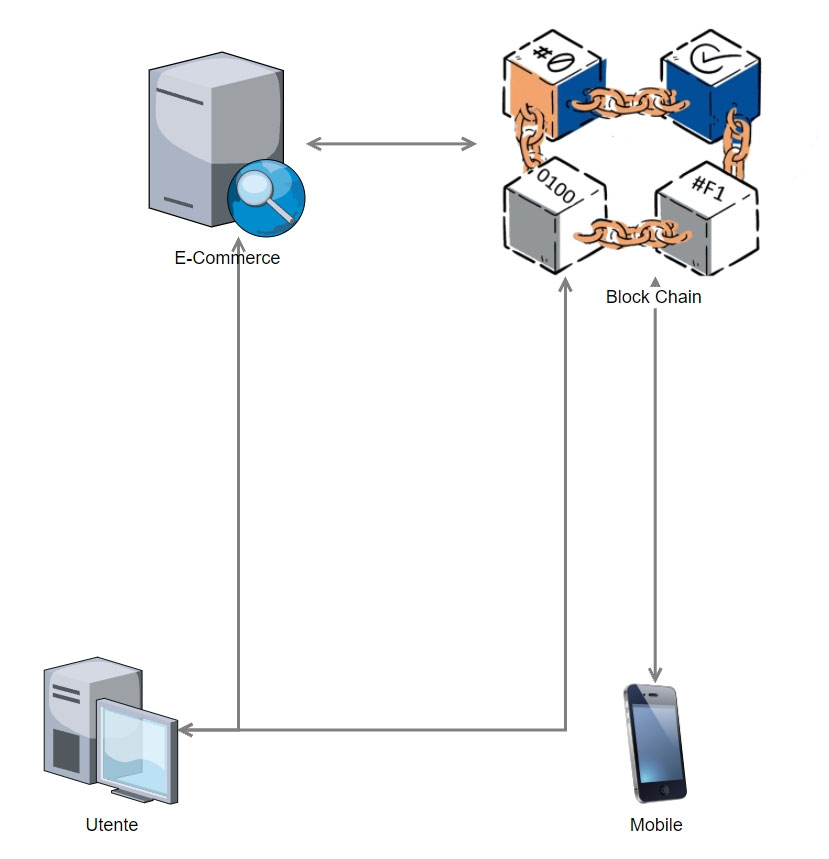
\includegraphics[scale=0.4]{Res/SyncLab.png}
        \caption{Pagamento sicuro e consegna garantita}
        \label{SyncLab}
    \end{figure}
    
    \subsection{Dominio}
        \subsubsection{Dominio Applicativo}
        
        Il capitolato si colloca nell’ambito degli acquisti online, dove da un lato c’è il compratore che desidera acquistare un bene mediante criptovaluta, dall’altro il venditore che vende un prodotto. Il luogo in cui le due parti si incontrano è un e-commerce.
        \subsubsection{Dominio Tecnologico}
        
        La Proponente preferisce non imporre tecnologie specifiche, ma resta aperta a nuove idee e proposte da parte dei fornitori del capitolato. Tuttavia esprime alcune scelte preferenziali da considerare nello svolgimento del progetto:	
        \begin{itemize}
		    \item  Utilizzo di Blockchain pubblica, come ad esempio Ethereum, con linguaggio \textit{Solidity} da usare per la scrittura degli smart contract; 
			\item Utilizzo di \textit{Java} e \textit{Angular} per lo sviluppo delle parti di Back-end e di Front-end della componente Web Application del sistema; 
			\item Utilizzo di database \textit{PostgreSQL}.
		\end{itemize}
    
    \subsubsection{Fattori Critici}
    I fattori critici su cui ci siamo soffermati ed ci hanno fatto desistere dall'intraprendere questo capitolato sono:
   \begin{itemize}
		\item Scarsa conoscenza da parte del gruppo della Blockchain così come della maggior parte delle tecnologie consigliate;
		\item Risulta difficile gestire il caso in cui un pacco sia smarrito;
		\item Nel caso in cui un pacco sia perso, occorre implementare dei meccanismi di rimborso del venditore da parte di chi si occupa della logistica;
		\item Non è possibile garantire l’anonimato dell’acquirente;
		\item Possono sorgere inconvenienti nel caso di rimborsi dovuti a prodotti malfunzionanti o indesiderati.
	\end{itemize}
    \subsection{Conclusioni}
    
    Inizialmente il gruppo ha preso in considerazione questa proposta. Tuttavia durante gli incontri che si sono tenuti sono emerse delle perplessità riguardanti l’effettiva fattibilità di questo capitolato. L’incontro tenutosi con l’azienda ha risposto solo parzialmente ai dubbi. Si è scelto quindi di escludere questo capitolato.
    
    
    
    
    
    
    
    
    
    
    
    
    
    
    
    
    
    
    
    
    
\section{Capitolato C3}
    \subsection{Informazioni generali} Informazioni generali
    \begin{itemize}
        \item \textbf{Nome}: CC4D
        \item \textbf{Proponente}: SanMarco Informatica
        \item \textbf{Committente}: Prof. Tullio Vardanega e Prof. Riccardo Cardin
    \end{itemize}
    \subsection{Descrizione} Descrizione
    
    Il progetto ha lo scopo di creare una web application, sia per mobile che per desktop,che
    permetta all’utente di gestire il controllo statistico dei processi di macchine produttive e 
    le relative caratteristiche da raccogliere in database e visualizzare su grafici.
    
    \subsection{Dominio} Dominio
        \subsubsection{Dominio Applicativo} Dominio Applicativo
        
        Il capitolato vuole portare il grupppo attraverso svariati strumenti e tecnologie a  creare un' API per l’immissione della misurazione di una determinata caratteristica, e la creazione di un motore di calcolo che, alla ricezione di una nuova misurazione, si occupi di metterla in relazione con le
        misurazioni precedenti al fine di calcolare se la serie di punti evidenza un processo “fuori controllo”.
        \subsubsection{Dominio Tecnologico} Dominio Tecnologico
        
        Per lo svolgimento del capitolato e per la creazione dell'applicatovo viene richiesta la conoscenza e la padronanzza delle seguenti tecnologie:
        \begin{itemize}
            \item \textit{NodeJS}: libreria JavaScript per la gestione del comportamento dell'applicativo;
            \item \textit{React}: per la parte front-end con js;
            \item \textit{Angular}: per il front-end;
            \item \textit{Git}: per il versionamento dell'applicativo.
        \end{itemize}
    
    \subsubsection{Fattori Critici} Fattori critici
    
    I fattori critici su cui ci siamo soffermati ed ci hanno fatto desistere dall'intraprendere questo capitolato sono:
    \begin{itemize}
            \item Molti temi di ambito differenti che richiedono un buon approfondimento;
            \item Spiegazione del capitolato troppa sintetica; 
            \item Moltitudine di requisiti obbligatori;
            \item Conoscere e dominare bene l'utilizzo di diverse tecnologie;
        \end{itemize}
    \subsection{Conclusioni} Conclusioni
    
    Il dominio applicativo dell'azienda appartiene ad un ambito che ha stimolato pochi di noi, non ci ha spinti verso l'assunzione del capitolato C3, ritenuto da noi molto valido nella sua interezza ma poco incline ai nostri interessi come gruppo.    
    
\newpage
    
\section{Capitolato C4}
    \subsection{Informazioni generali} Informazioni generali
    \begin{itemize}
        \item \textbf{Nome}: Guida Michelin @ social
        \item \textbf{Proponente}: ZERO12
        \item \textbf{Committente}: Prof. Tullio Vardanega e Prof. Riccardo Cardin
    \end{itemize}
    \subsection{Descrizione} Descrizione
    
    L’azienda committente chiede di realizzare una piattaforma che sia una sorta di guida Michelin. Lo scopo dovrebbe essere quindi quello di creare una classifica dei posti di maggiore interesse analizzando i contenuti social prelevati dai social network Instagram e TikTok, e incrociando i risultati ottenuti con le recensioni online. A tale scopo, la piattaforma deve essere in grado di estrapolare dai social informazioni utili a determinare se un posto è giudicato positivamente o negativamente, partendo da ciò che viene condiviso (come commenti testuali, messaggi vocali, immagini, ecc...).
    
    \begin{figure}[h!]
        \centering
        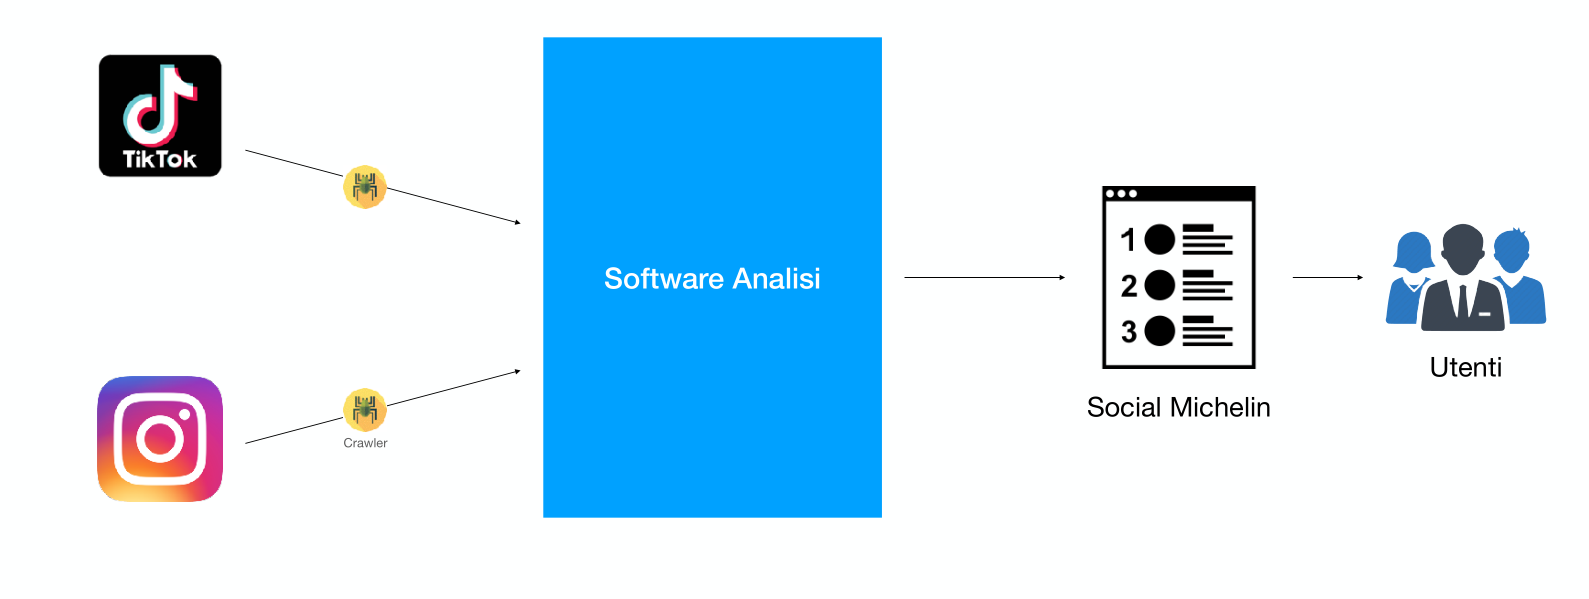
\includegraphics[scale=0.4]{Res/C4.PNG}
        \caption{Ottenimento info dai social}
        \label{GuidaMIchelin}
    \end{figure}
    
    \subsection{Dominio} Dominio
        \subsubsection{Dominio Applicativo} Dominio Applicativo
        
        Il capitolato si colloca nell'ambito dei social network.
        Esso vuole offrire ai propri utenti un' esperienza più avvincente possibile utilizzando i contenuti creati pubblicamente dai vari utilizzatori dei social Network, in prevalenza TikTok e Instagram.
        \subsubsection{Dominio Tecnologico} Dominio Tecnologico
        
        Il committente raccomanda di utilizzare la tecnologia di Amazon Web Services ed in particolare i seguenti servizi:
		\begin{itemize}
			\item \textit{AWS Fargate}: servizio Serverless per la gestione a container;
			\item \textit{AWS AppSync}: servizio gestito per lo sviluppo rapido di API GraphQL;
			\item \textit{Neptune}: database a grafo ideale per tracciare per questo tipo di progetti e tracciare efficientemente le relazioni tra i dati.
		\end{itemize}
		I linguaggi di programmazione da utilizzare sono:
		\begin{itemize}
			\item \textit{NodeJS}: linguaggio di programmazione per lo sviluppo di API Restful JSON a supporto dell’applicativo;
			\item \textit{Swift}: linguaggio di programmazione per lo sviluppo di app in ambito iOS/MacOS;
			\item \textit{Kotlin}: linguaggio di programmazione per lo sviluppo di app in ambito Android.
		\end{itemize}
		Inoltre l’architettura deve essere basata a micro-servizi.
    
    \subsubsection{Fattori Critici} Fattori critici
    I fattori critici su cui ci siamo soffermati ed ci hanno fatto desistere dall'intraprendere questo capitolato sono:
    \begin{itemize}
            \item A primo impatto il gruppo si è mostrato scettico sul fatto che, secondo le normative sui dati vigenti di Instagram e TikTok, sia possibile raccogliere i dati degli utenti;
			\item Il capitolato, vista la complessità, risulta essere particolarmente dispendioso in termini di tempo;
			\item Poca esperienza su AWS così come sui linguaggi di programmazione da utilizzare.
        \end{itemize}
    \subsection{Conclusioni} Conclusioni
    
    Il dominio applicativo dell'azienda appartiene ad un ambito che ha stimolato pochi di noi, non ci ha spinti verso l'assunzione del capitolato C4, ritenuto da noi molto valido nella sua interezza ma poco incline ai nostri interessi come gruppo, il capitolato è stato poi scartato anche per via dei molti punti poco chiari.

\newpage

\section{Capitolato C6}
    \subsection{Informazioni generali} Informazioni generali
    \begin{itemize}
        \item \textbf{Nome}: Smart4Energy – A new way in energy monitoring and control
        \item \textbf{Proponente}: Socomec Innovative Power Solutions
        \item \textbf{Committente}: Prof. Tullio Vardanega e Prof. Riccardo Cardin
    \end{itemize}
    \subsection{Descrizione} Descrizione
    
    Il progetto ha lo scopo di cambiare il modo in cui le persone si interfacciano ai dispositivi Socomec e il modo in
    cui viene erogato il servizio di assistenza.
    
    Per poter quindi fornire ausilio per un avanzamento tecnologico ai gurppi di continuità (UPS), per far si che possano essere fruiti ed utilizzati, tramite diverse tecnologie, da differenti device.
    
    
    \subsection{Dominio} Dominio
        \subsubsection{Dominio Applicativo} Dominio Applicativo
        
        Il capitolato vuole soddisfare una nuova esigenza nell'ambito dell'UPS derivata dai consumatori.
        Il capitolato vuole proporre all’utente una nuova esperienza d’uso tramite il dispositivo, smartphone o
        tablet, dell’utente stesso.
        In questo modo l’utente sarà naturalmente a suo agio, utilizzando il proprio device per svolgere operazioni riguardanti l'unità di UPS.
        \subsubsection{Dominio Tecnologico} Dominio Tecnologico
        
        Per lo svolgimento del capitolato e per la creazione dell'applicatovo che si interfaccierebbe con l'unità di UPS, viene richiesta la conoscenza dell'ambito mobile, per poter lavorare con apparati mobili che sono dotati, nella quasi totalità, di sistema operativo Android™ o iOS™.
        \begin{itemize}
            \item \textit{Kotlin}: un moderno linguaggio di programmazione lato mobile sviluppato da JetBrains ed in elevata ascesa;
            \item \textit{Java}: dato che i sistemi Android™ sono da sempre stati programmati in Java, per permetterci quindi la più alta configurazione possibile;
            \item \textit{Swift}: per la parte di programmazione relativa ad iOS™;
            \item \textit{Git}: per il versionamento dell'applicativo.
        \end{itemize}
    
    \subsubsection{Fattori Critici} Fattori critici
    I fattori critici su cui ci siamo soffermati ed ci hanno fatto desistere dall'intraprendere questo capitolato sono:
    \begin{itemize}
            \item Molti di noi non hanno familiarità con le tecnologie proposte;
            \item Il fatto che l'azienda proponente abbia come main operativo un campo differente dal nostro; 
            \item Capitolato troppo lungo e dispersivo.
        \end{itemize}
    \subsection{Conclusioni} Conclusioni
    
    Il dominio applicativo dell'azienda appartiene ad un ambito che ha stimolato pochi di noi, non ci ha spinti verso l'assunzione del capitolato C6, ritenuto da noi molto valido nella sua intereza ma poco incline ai nostri interessi come gruppo.
    
    \begin{figure}[h!]
        \centering
        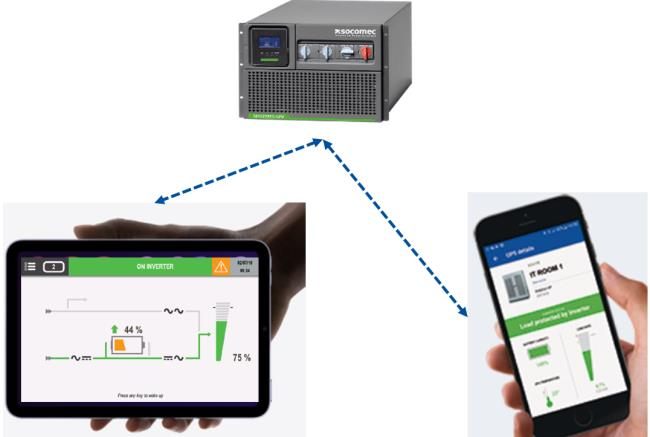
\includegraphics[scale=0.4]{Res/SocomecConnection.png}
        \caption{Connesione dei dispositivi}
        \label{socom}
    \end{figure}

\end{document}
